% !TEX root = 99_main.tex

An experiment was conducted in indoor and outdoor spaces around Singapore. Most of the participants were working at the National University of Singapore (NUS) and using several flexible work spaces around campus. Fifteen participants were recruited for the experiment and equipped with a Fitbit Versa or Ionic watch. The \emph{cozie} clock-face was installed and set to request thermal preference (prefer warmer, prefer cooler, comfy), and the set to request feedback up to five times per day at regular intervals. These feedback requests take the form of a gentle vibration of the watch to prompt the user to provide feedback.
% at the hours of 9:00, 11:00, 13:00, 15:00, and 17:00. 

The watch was further complimented with Internet-of-Things (IoT) connected on-body and environmental sensors. The on-body sensor consists of a temperature and light sensor from \emph{mbient-labs}\footnote{\url{https://mbientlab.com/}} that had been modified to fit the watch strap with a custom 3D printed case. An off-body sensor measuring temperature and humidity was attached to the participants bag. The sensors communicate via Bluetooth to Raspberry-Pi gateways that had been positioned throughout the working space. Data from the cozie watch face, and the environmental sensors were aggregated in an Influx cloud time-series database, which served as a platform for data acquisition and fault detection. 
% Source codes can be found here \cite{aurek-data}.


% \begin{figure}
% \begin{center}
% 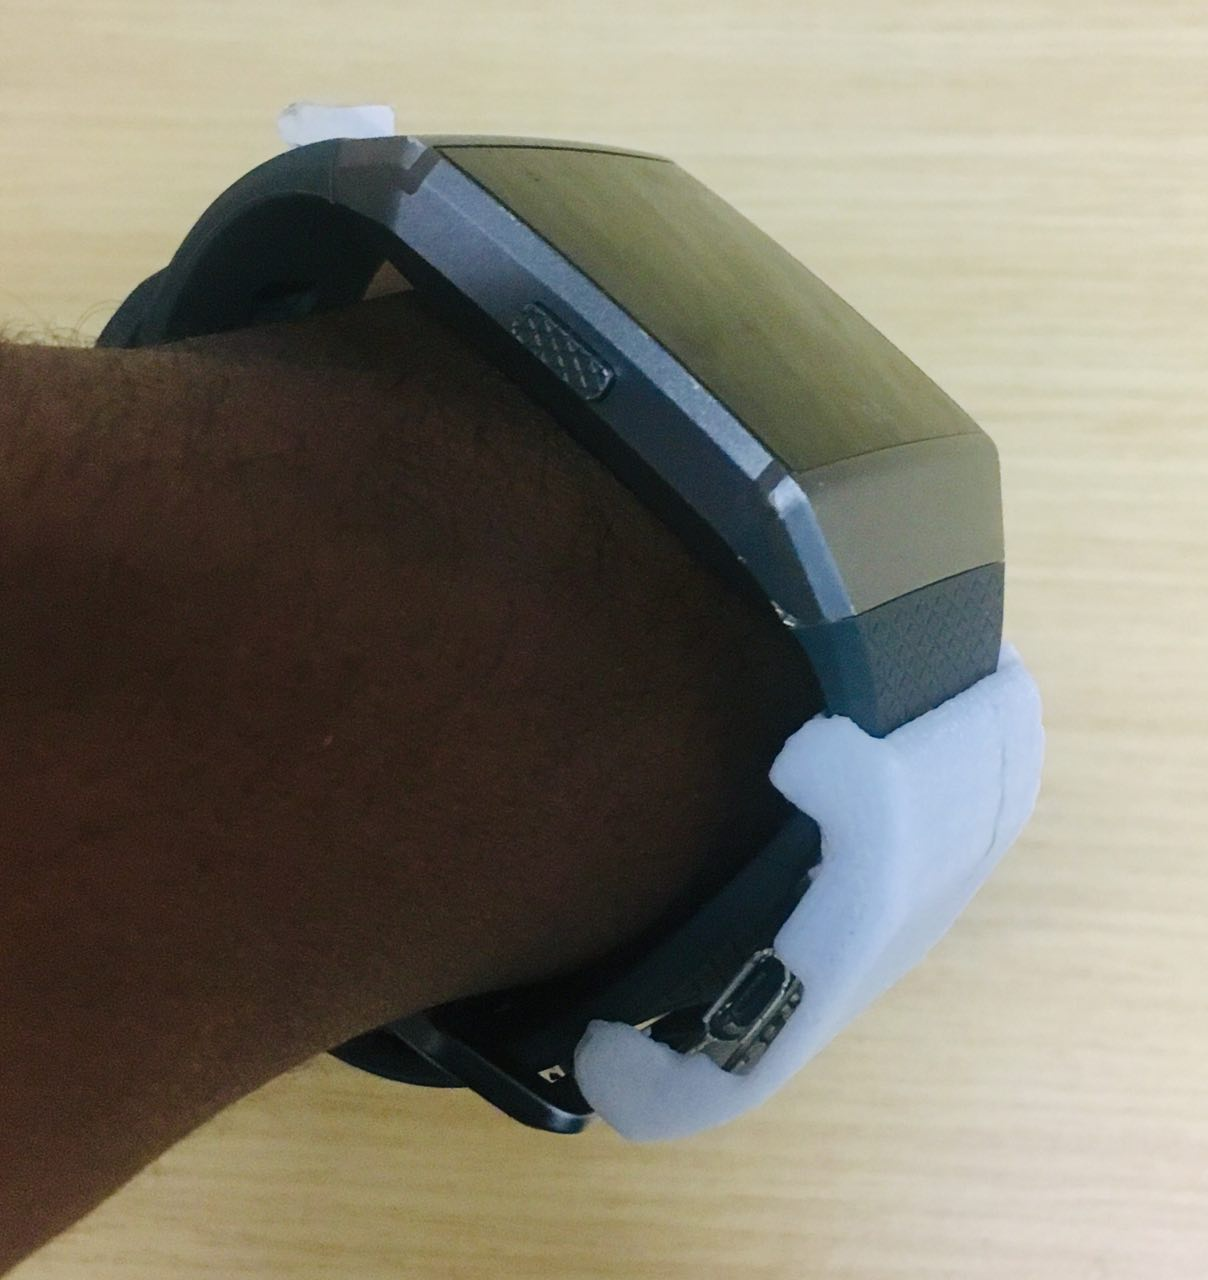
\includegraphics[width=0.2\textwidth, trim= 0cm 0cm 0cm 0cm,clip]{strap-pack.jpg}
% \caption{Strap-Pack}
% \label{fig:strappack}
% \end{center}
% \end{figure}

